% !TeX program = xelatex
\documentclass[12pt, a4paper]{article}

% Font i podrška za srpsku ćirilicu (XeLaTeX/LuaLaTeX)
\usepackage{fontspec}
% Pri učitavanju sistemskih fontova fontspec podrazumevano isključuje
% TeX ulazne ligature, pa se `---` prikazuje kao tri crtice umesto crte (—).
% Ovo ih ponovo uključuje za sve fontove (i ćirilične familije ispod).
\defaultfontfeatures{Ligatures=TeX}
\setmainfont{Times New Roman}
\setsansfont{Arial}
\setmonofont{Courier New}

\usepackage{polyglossia}
\setmainlanguage{serbianc}

% Times New Roman/Arial/Courier New imaju ćirilične glifove, ali ne deklarišu
% OpenType "cyrl" script tag, pa ga polyglossia ne prepoznaje automatski.
% Eksplicitno vezujemo ćirilične familije fontova da bi se ćirilica
% ispravno renderovala (inače polyglossia baca grešku i tekst izlazi pogrešno).
\newfontfamily\cyrillicfont{Times New Roman}
\newfontfamily\cyrillicfontsf{Arial}
\newfontfamily\cyrillicfonttt{Courier New}

\usepackage{graphicx}
\graphicspath{ {images/} }

% Za matematičke jednačine
\usepackage{amsmath}
\usepackage{amssymb}
\DeclareMathOperator*{\minimize}{minimize}
\newcommand{\norm}[1]{\lVert#1\rVert_2}
\usepackage{multirow} % za više redova u jednoj ćeliji tabele

% Za prikaz koda
\usepackage{listings}

% Za slike jednu pored druge
\usepackage{subcaption}
% Za slike i tekst jedan pored drugog
\usepackage{wrapfig}

% Hiperlinkovi iz sadržaja
\usepackage{hyperref}
\hypersetup{
    colorlinks,
    citecolor=red,
    filecolor=black,
    linkcolor=blue,
    urlcolor=black
}

% Bibliografija
\usepackage[
    backend=biber,
    style=numeric,
    sorting=none
]{biblatex}
\addbibresource{references.bib}
\usepackage{csquotes}

% Дијаграми (TikZ)
\usepackage{tikz}
\usetikzlibrary{arrows.meta, positioning, calc, decorations.pathreplacing}
\usepackage{pgfplots}
\pgfplotsset{compat=1.18}

% Margine
\usepackage[left=3cm, right=2.5cm, top=2.5cm, bottom=2.5cm]{geometry}

% Automatski prelazak na novu stranu na početku svake sekcije
\usepackage{titlesec}
\newcommand{\sectionbreak}{\clearpage}

% Početna numeracija stranica je rimska
\pagenumbering{roman}

\begin{document}

%%%%%%%%%%%%%%%%%%%%%%%%%%%%%%%%%%%%%%%%%%%%%%%%%%%%%%%%%% NASLOVNA STRANA %%%%%%%%%%%%%%%%%%%%%%%%%%%%%%%%%%%%%%%%%%%%%%%%%%%%%%%%%
\begin{titlepage}
\centering

\includegraphics[width=0.2\textwidth]{ETF_logo}\par
\vspace{1cm}
{\LARGE\MakeUppercase{Електротехнички факултет}\par}
{\LARGE\MakeUppercase{Универзитет у Београду}\par}
\vspace{1cm}
{\Large\MakeUppercase{Дипломски рад}\par}
\vspace{0.5cm}
{\huge\bfseries Испитивање границе учења имитацијама у симулационом окружењу за роботско извршавање високо прецизних задатака\par}
\vspace{2cm}
{\large\itshape Кандидат\par}
{\large\itshape Михајло Стевановић\par}
{\large\itshape Број индекса: 2022/0315\par}
\vfill
{\large\itshape Ментор\par}
{\large\itshape Проф. др Коста Јовановић\par}
\vfill
{\large \today \par}
\end{titlepage}

%%%%%%%%%%%%%%%%%%%%%%%%%%%%%%%%%%%%%%%%%%%%%%%%%%%%%%% ПРЕДГОВОР %%%%%%%%%%%%%%%%%%%%%%%%%%%%%%%%%%%%%%%%%%%%%%%%%%%%%%%%
\addcontentsline{toc}{section}{Предговор}
\section*{Предговор}

Овај рад настао је у Лабораторији за роботику Електротехничког факултета Универзитета у Београду, смештеној у Палати науке, као наставак студентске праксе коју је аутор претходно реализовао у истој лабораторији, под менторством проф.\ др Косте Јовановића.

Истраживање је спроведено у оквиру учешћа лабораторије на такмичењу Intrinsic AI for Industry Challenge, које организује компанија Intrinsic (Alphabet Inc.), а које је усмерено на задатке прецизне роботске манипулације у индустријском контексту.
Рад је део ширег тимског пројекта посвећеног аутоматској инсерцији кабла у конекторски порт.
У оквиру тог пројекта, развој скриптоване oracle политике и прикупљање скупа демонстрација реализовао је колега \textit{(Добрица Јанковић)}; ова теза се, на тако прикупљеним демонстрацијама, фокусира на експерименталну студију метода учења имитацијама (ACT и Diffusion Policy).

\clearpage

%%%%%%%%%%%%%%%%%%%%%%%%%%%%%%%%%%%%%%%%%%%%%%%%%%%%%%% ЗАХВАЛНИЦА %%%%%%%%%%%%%%%%%%%%%%%%%%%%%%%%%%%%%%%%%%%%%%%%%%%%%%%%
\addcontentsline{toc}{section}{Захвалница}
\section*{Захвалница}

Желим да изразим искрену захвалност проф.\ др Кости Јовановићу на указаном поверењу и прилици да своју студентску праксу, а потом и дипломски рад, реализујем у лабораторији Електротехничког факултета у Палати Науке.
Рад у том окружењу пружио ми је непроцењиво практично искуство и непосредан увид у процес научноистраживачког рада.

Посебну захвалност дугујем својим менторима, Давиду Сеничићу и др Филипу Бечановићу, на издвојеном времену, стрпљењу и знању које су несебично делили са мном током рада на овом пројекту.
Захваљујући њиховим упутствима, конкретним референцама и правовременим смерницама успео сам да попуним кључне празнине у знању и да рад доведем до краја.

Захваљујем се и свим сарадницима лабораторије за роботику на колегијалном радном окружењу и свакодневној размени идеја.

\vspace{1.5cm}
\noindent Михајло Стевановић

\noindent У Београду, јун 2026.\ године

\clearpage

%%%%%%%%%%%%%%%%%%%%%%%%%%%%%%%%%%%%%%%%%%%%%%%%%%%%%%% САДРЖАЈ %%%%%%%%%%%%%%%%%%%%%%%%%%%%%%%%%%%%%%%%%%%%%%%%%%%%%%%%
\tableofcontents

%%%%%%%%%%%%%%%%%%%%%%%%%%%%%%%%%%%%%%%%%%%%%%%%%%%%%%%%%% УВОД %%%%%%%%%%%%%%%%%%%%%%%%%%%%%%%%%%%%%%%%%%%%%%%%%%%%%%%%%%
\section{Увод}
\label{sec:uvod}
\pagenumbering{arabic}
Савремена индустријска аутоматизација суочава се са растућом потребом за роботским системима способним да извршавају задатке прецизне монтаже (енгл.\ \textit{assembly}) које је, до скора, могуће обавити искључиво уз помоћ руке оператора.
Кабловска инфраструктура, коју чине конектори, кабловске везице и сродни савитљиви елементи, незаобилазна је у производним линијама аутомобилске, ваздухопловне и медицинске индустрије.
Упркос дугогодишњем напретку у роботској манипулацији, аутоматско уметање кабла у конекторски порт остаје нерешен проблем и директно ограничава степен аутоматизације у производним погонима.

Овај задатак представља парадигматски пример такозваног проблема деформабилних линеарних објеката (енгл.\ \textit{deformable linear objects}, DLO).
За разлику од крутих тела, кабл испољава комплексну механику деформације која се не може поуздано унапред предвидети: чак и при идентичним почетним условима, конфигурација кабла у простору варира на начин неподложан аналитичком моделовању.
Истовремено, успешна инсерција захтева прецизност на нивоу неколико милиметара, свако одступање завршног механизма (енгл.\ \textit{end-effector}) изнад те границе резултира неуспехом задатка.
Ова комбинација непредвидивости деформације и захтеване прецизности чини аутоматско уметање кабла једним од отворених проблема индустријске роботике.

Овај рад настао је у оквиру учешћа на такмичењу Intrinsic AI for Industry Challenge, које организује компанија Intrinsic (Alphabet Inc.), а које је усмерено на задатке прецизне роботске манипулације у индустријском контексту.
За потребе учесника, Intrinsic је обезбедио потпуно конфигурисано симулационо окружење.
Оно обухвата платформу NVIDIA Isaac Sim за физичку симулацију и фотореалистично приказивање сцене засновано на графичким процесорима (енгл.\ \textit{GPU}), уз праћење зрака (енгл.\ \textit{ray tracing}); OpenUSD склопове за дефиницију сцене, робота и задатка; те Docker контејнер са свим потребним библиотекама унапред инсталираним и међусобно усклађеним, из ког је могуће директно покретати симулације и тренирати политике.
Оваква стандардизована поставка елиминисала је проблем конфигурације окружења и обезбедила потпуно репродуцибилне услове за систематско поређење метода.

Класични приступи решавању проблема DLO манипулације заснивају се на експлицитном моделовању геометрије и динамике кабла те планирању путање на основу тог модела.
Ови приступи носе високу рачунарску цену и остају осетљиви на грешке услед немоделованог понашања.
Као алтернатива, у овом раду истражују се методе \textit{учења имитацијама} (енгл.\ \textit{imitation learning}, IL), парадигма у којој агент политику (пресликавање опсервација у акције) учи директно из демонстрација стручног агента, без потребе за експлицитним моделом динамике окружења.
Конкретно, поређене су две савремене IL архитектуре: Action Chunking with Transformers (ACT)~\cite{zhao2023act} и Diffusion Policy (DP)~\cite{chi2023diffusionpolicy}, обе у формулацији клонирања понашања (енгл.\ \textit{behavioral cloning}, BC).
Скуп демонстрација прикупљен је путем такозване \textit{oracle политике}, скриптованог агента заснованог на коначном аутомату (енгл.\ \textit{state machine}) коме је, за разлику од тренираних политика, омогућен привилегован приступ апсолутним координатама циљног порта у симулационом окружењу.
Ова политика развијена је у оквиру ширег истраживачког пројекта и у овом раду представља фиксну, унапред дату компоненту тока података; њена интерна имплементација стога није предмет ове студије, већ се користи као стандардизован извор демонстрација.
Тренирани модели ту информацију не поседују, већ уче искључиво из опсервација (RGB слике камере, позиција завршног механизма) и акција које је oracle извршио, чиме је задатак учења реалистично отежан у складу са ограничењима стварних роботских система.

\subsection{Циљеви рада и истраживачка питања}
\label{subsec:ciljevi}
Централно истраживачко питање рада гласи: \textit{колико далеко, и под којим условима, методе учења имитацијама могу да достигну задовољавајући ниво перформанси на задатку с милиметарском прецизношћу?}
Из овог општег питања изведени су следећи циљеви рада:
\begin{enumerate}
    \item[\textbf{Ц1.}] Одредити оквирни минималан број демонстрација потребан да модел достигне прихватљив проценат успешности (енгл.\ \textit{success rate}).
    \item[\textbf{Ц2.}] Упоредити скалабилност архитектура ACT и Diffusion Policy у односу на величину скупа података за обуку.
    \item[\textbf{Ц3.}] Испитати утицај аугментације података и синтетичког шума на опсервације на робустност и способност генерализације политике.
    \item[\textbf{Ц4.}] Идентификовати „плафон" перформанси ових метода на задатку овог типа и детерминисати факторе који га одређују.
\end{enumerate}

\subsection{Допринос рада}
\label{subsec:doprinos}
Допринос овог рада је троструки.
Прво, пружа се систематска експериментална студија граница двеју савремених IL метода на задатку високе прецизности, у контролисаном симулационом окружењу и над демонстрацијама прикупљеним заједничком oracle политиком.
Друго, анализира се зависност перформанси од величине скупа података и одређује оквирни минималан број демонстрација неопходан за прихватљив проценат успешности.
Треће, квантификује се утицај аугментације и додатог шума на перформансе, пружајући смернице за практичну примену IL метода у индустријским условима.

\subsection{Структура рада}
\label{subsec:struktura}
Рад је организован на следећи начин.
Поглавље~\ref{sec:pregled_literature} даје преглед релевантне литературе из области учења имитацијама, са посебним освртом на ACT и Diffusion Policy, као и сродне радове о роботској манипулацији деформабилним објектима.
У Поглављу~\ref{sec:metodologija} описују се формулација проблема, архитектуре модела и ток података, укључујући заједничку oracle политику као контекст у коме настаје скуп демонстрација.
Поглавље~\ref{sec:eksperimentalna_postava} детаљно излаже симулационо окружење, простор опсервација и акција, хиперпараметре и метрике евалуације.
Резултати свих експерименталних димензија приказани су у Поглављу~\ref{sec:rezultati}, а њихова интерпретација и ограничења дискутовани у Поглављу~\ref{sec:diskusija}.
Поглавље~\ref{sec:zakljucak} доноси закључна разматрања и правце будућих истраживања.
%%%%%%%%%%%%%%%%%%%%%%%%%%%%%%%%%%%%%%%%%%%%%%%%%%%%%%%% ПРЕГЛЕД ЛИТЕРАТУРЕ %%%%%%%%%%%%%%%%%%%%%%%%%%%%%%%%%%%%%%%%%%%%%%%%%%%%
\section{Преглед литературе}
\label{sec:pregled_literature}

\subsection{Учење имитацијама и клонирање понашања}
\label{subsec:il_bc}

Учење имитацијама (IL) је парадигма у оквиру које агент стиче политику $\pi$ опонашањем стручног демонстратора, без директног дефинисања функције награде окружења.
Најједноставнији облик IL-а је клонирање понашања (BC), уведено у контексту аутономне навигације у систему ALVINN~\cite{pomerleau1989alvinn}.
У BC формулацији, политика се тренира надгледаним учењем на скупу демонстрација $\mathcal{D} = \{(\mathbf{o}_t, \mathbf{a}_t)\}_{t=1}^{T}$:

\begin{equation}
    \pi^* = \arg\min_\pi \;\mathbb{E}_{(\mathbf{o},\,\mathbf{a})\,\sim\,\mathcal{D}}\bigl[\mathcal{L}\bigl(\pi(\mathbf{o}),\,\mathbf{a}\bigr)\bigr],
    \label{eq:bc_objective}
\end{equation}

\noindent где $\mathbf{o}$ означава опсервацију, $\mathbf{a}$ акцију стручног агента, а $\mathcal{L}$ критеријумску функцију губитка.

Кључно ограничење BC-а је проблем акумулације грешке: мала одступања у предвиђеним акцијама нагомиланим ефектом одводе агента у стања која нису покривена скупом демонстрација, а политика нема усвојеног понашања за реоријентацију и поправку из таквих стања.
Овај феномен, познат као \textit{distribution shift}, математички је формализовао Ross et al.~\cite{ross2011dagger}, а у истом раду предложен је алгоритам DAgger (Dataset Aggregation), који скуп демонстрација итеративно обогаћује стањима насталим током евалуације (енгл.\ \textit{rollout}) тренираног агента.
Свеобухватна студија Mandlekar et al.~\cite{mandlekar2021robomimic} на скупу референтних задатака Robomimic (енгл.\ \textit{benchmark}) показала је да на успешност BC-а у роботској манипулацији пресудно утичу квалитет и покривеност простора стања у демонстрацијама, а не искључиво архитектура модела.
У истом духу, Belkhale et al.~\cite{belkhale2023dataquality} показују да обим и квалитет скупа демонстрација често одређују горњу границу перформанси више него сам избор алгоритма, што непосредно мотивише питање колико је демонстрација заиста потребно за прихватљив проценат успешности (циљ Ц1).

\subsection{Action Chunking with Transformers (ACT)}
\label{subsec:act}

ACT је метода учења имитацијама коју су предложили Zhao et al.~\cite{zhao2023act} за задатке прецизне биманипулације.
Централни допринос је концепт \textit{action chunking}-а: уместо предвиђања јединичне акције у сваком временском кораку, политика предвиђа блок (chunk) од $k$ узастопних акција $(\mathbf{a}_t, \mathbf{a}_{t+1}, \ldots, \mathbf{a}_{t+k-1})$.
Ефективни хоризонт задатка тако се смањује за фактор $k$, чиме се директно ублажава проблем акумулације грешке~\cite{ross2011dagger}, будући да политика уместо $T$ независних одлука доноси свега $\lceil T/k \rceil$.

Архитектура ACT-а комбинује условни варијациони аутоенкодер (CVAE) и кодер-декодер трансформер~\cite{vaswani2017attention} (Сл.~\ref{fig:act_arch}):

\begin{itemize}
    \item \textbf{CVAE кодер} (активан искључиво током тренинга): прима секвенцу акција из демонстрације и тренутне позиције зглобова, те их сажима у латентну променљиву $\mathbf{z} \sim \mathcal{N}(\boldsymbol{\mu}, \mathrm{diag}(\boldsymbol{\sigma}^2))$.
    Улога CVAE-а је моделовање вишемодалности у демонстрацијама, при чему се различити стилови извршавања истог задатка кодирају у различите вредности $\mathbf{z}$.
    У фази примене, CVAE кодер се изоставља, а вредност латентног вектора $\mathbf{z}$ поставља на нулу.
    \item \textbf{Трансформерски декодер}: прима визуелне карактеристике $N$ RGB камера (кодоване ResNet-18~\cite{he2016resnet} кичмом), позиције зглобова и $\mathbf{z}$, те унакрсним механизмом пажње генерише предвиђени блок акција.
    Дизајн декодера заснован је на DETR~\cite{carion2020detr} архитектури са учивим позиционим кодовима у улози упитних вектора.
\end{itemize}

\begin{figure}[htbp]
    \centering
    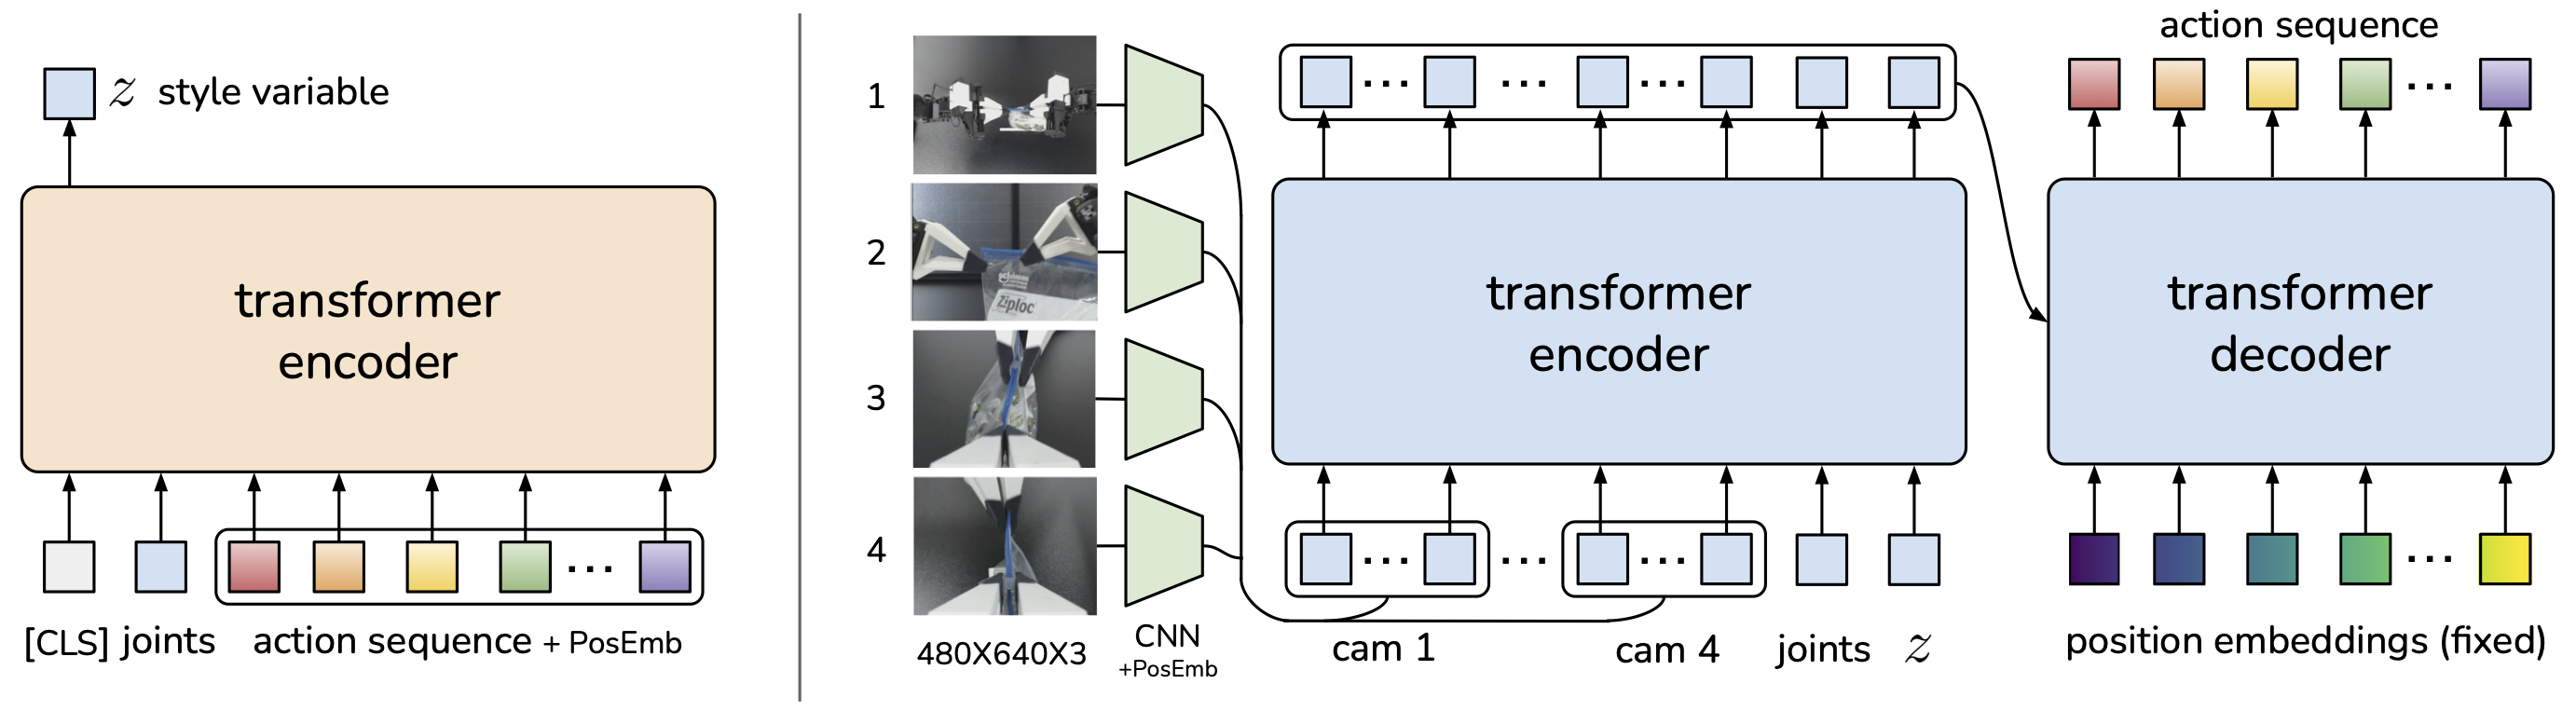
\includegraphics[width=\linewidth]{act_arhitektura}
    \caption{Архитектура ACT политике: CVAE кодер (лево) сажима секвенцу акција и позиције зглобова у латентну променљиву $\mathbf{z}$, док трансформерски кодер-декодер (десно) на основу слика камера, позиција зглобова и $\mathbf{z}$ предвиђа секвенцу акција. Преузето из~\cite{zhao2023act}.}
    \label{fig:act_arch}
\end{figure}

Критеријумска функција током тренинга комбинује L1 реконструкцијску грешку и KL регуларизацију:

\begin{equation}
    \mathcal{L}_{\mathrm{ACT}}
    = \mathbb{E}\bigl[\|\hat{\mathbf{a}} - \mathbf{a}\|_1\bigr]
    + \beta \cdot D_{\mathrm{KL}}\!\bigl(\mathcal{N}(\boldsymbol{\mu},\,\boldsymbol{\sigma}^2\mathbf{I})\,\|\,\mathcal{N}(\mathbf{0},\,\mathbf{I})\bigr),
    \label{eq:act_loss}
\end{equation}

\noindent где је $\beta$ хиперпараметар (подразумевано $\beta = 10$) који уравнотежује прецизност предвиђања и регуларизацију латентног простора.

За глаткост покрета при преклапајућим акцијским блоковима, ACT опционо примењује временско усредњавање (енгл.\ \textit{temporal ensembling}): предвиђања за исти тренутак из вишеструких узастопних очитавања политике комбинују се са експоненцијалним тежинама $w_i = e^{-m\cdot i}$.
На задацима прецизне биманипулације у физичком окружењу ACT постиже успешност 80–96\%~\cite{zhao2023act}, уз значајно надмашивање референтних метода BC-ConvMLP, BeT и VINN.
Аблациона студија у истом раду показала је да само повећање величине блока са $k{=}1$ на $k{=}100$ побољшава успешност са 1\% на 44\% на репрезентативном задатку биманипулације.

\subsection{Diffusion Policy}
\label{subsec:dp}

Diffusion Policy (DP) је метода учења политике коју су увели Chi et al.~\cite{chi2023diffusionpolicy}, заснована на одшумљавању дифузијским вероватносним моделима (DDPM)~\cite{ho2020ddpm} примењеним на простор акција роботске политике.
Кључна идеја је представљање условне расподеле акција $p(\mathbf{A}_t \mid \mathbf{O}_t)$ кроз итеративни поступак уклањања шума:

\begin{equation}
    \mathbf{x}^{(k-1)} = \alpha\!\left(\mathbf{x}^{(k)} - \gamma\,\boldsymbol{\epsilon}_\theta\!\bigl(\mathbf{x}^{(k)},\,k,\,\mathbf{O}_t\bigr)\right) + \boldsymbol{\eta}, \quad \boldsymbol{\eta} \sim \mathcal{N}(\mathbf{0},\,\sigma^2\mathbf{I}),
    \label{eq:dp_denoising}
\end{equation}

\noindent где $\mathbf{x}^{(K)}$ представља иницијални Гаусов шум, а $\boldsymbol{\epsilon}_\theta$ мрежу тренирану да предвиди шум условљен опсервацијом $\mathbf{O}_t$.
Поступак поступно претвара насумичан шум у кохерентан акцијски план кроз $K$ корака одшумљавања.
Применом DDIM~\cite{song2021ddim} шеме потребан број ових корака смањује се са 100 на свега 10, чиме се постиже кашњење испод 0,1\,с при примени политике на GPU.

DP такође предвиђа секвенце акција ($T_p$ корака), али извршава само $T_a < T_p$ пре следеће активације политике, остварујући баланс дугорочног планирања и брзе реакције на тренутне опсервације.
Предложена су два архитектурална варијанта (Сл.~\ref{fig:dp_arch}):

\begin{itemize}
    \item \textbf{Conv-DP}: 1D временске конволуције са Feature-wise Linear Modulation (FiLM)~\cite{perez2018film} за условљавање опсервацијама; поуздан у широком спектру задатака.
    \item \textbf{Trans-DP}: transformer decoder блокови са каузалним маскирањем пажње; надмашује Conv-DP на задацима са нагло променљивим и вишемодалним акцијама.
\end{itemize}

\begin{figure}[htbp]
    \centering
    \resizebox{\linewidth}{!}{%
    \begin{tikzpicture}[
        font=\small,
        >={Stealth[length=2.2mm]},
        big/.style={draw, rounded corners=3pt, align=center, fill=orange!18, inner sep=6pt, minimum height=15mm},
        blk/.style={draw, rounded corners=2pt, align=center, fill=blue!12, inner sep=4pt, minimum height=9mm},
        film/.style={draw, rounded corners=2pt, align=center, fill=green!16, inner sep=4pt, minimum height=9mm},
        tok/.style={draw, minimum size=9mm, inner sep=1pt, align=center, font=\scriptsize},
        pcap/.style={font=\footnotesize\bfseries},
        lbl/.style={font=\footnotesize\itshape},
        brace/.style={decorate, decoration={brace, amplitude=4pt}}
    ]
        %=================== ПАНЕЛ а) Општа формулација ===================
        % токени опсервације
        \node[tok, fill=blue!22] (o1) {$\mathbf{o}_{t-1}$};
        \node[tok, fill=blue!38, right=0.7mm of o1] (o2) {$\mathbf{o}_t$};
        \node[lbl, below=1.5mm of o1.south] (olab) {$\mathbf{O}_t$\;($n_{\mathrm{obs}}$ корака)};
        % DP блок
        \node[big, right=11mm of o2] (dp) {Diffusion Policy\\[2pt]$\boldsymbol{\epsilon}_\theta(\mathbf{O},\mathbf{A},k)$};
        \draw[->,thick] (o2) -- (dp);
        % токени акцијске секвенце
        \node[tok, fill=red!25, right=12mm of dp] (a1) {$\mathbf{a}_t$};
        \node[tok, fill=orange!32, right=0.7mm of a1] (a2) {$\mathbf{a}_{t+1}$};
        \node[tok, fill=yellow!45, right=0.7mm of a2] (a3) {$\mathbf{a}_{t+2}$};
        \node[tok, fill=green!30, right=0.7mm of a3] (a4) {$\cdots$};
        \node[lbl, above=1.5mm of a2.north east] {Акцијска секвенца $\mathbf{A}_t$};
        \draw[->,thick] (dp) -- (a1);
        \draw[brace] (a4.south east) -- (a1.south west)
            node[midway, below=4pt, lbl] {хоризонт предвиђања $T_p$};
        \node[pcap] at ([yshift=-25mm]$(o1.west)!0.5!(a4.east)$) {а) Општа формулација};

        %=================== раздвојна линија ===================
        \draw[dashed] ($(a4.east)+(11mm,22mm)$) -- ($(a4.east)+(11mm,-27mm)$);

        %=================== ПАНЕЛ б) Конволуциона варијанта ===================
        % условљавање
        \node[big, right=20mm of a4, text width=20mm, minimum height=20mm] (cond)
            {Опсервација $\mathbf{O}_t$\\[2pt]\footnotesize (условљавање)};
        % FiLM + Conv1D јединица
        \node[film, right=17mm of cond] (axb) {$a\,\mathbf{x}+b$\\[1pt]\footnotesize FiLM};
        \node[tok, fill=violet!22, below=7mm of axb, minimum width=20mm] (xemb) {$\mathbf{x}$: Action Emb};
        \node[blk, right=9mm of axb] (conv) {Conv1D};
        \node[tok, fill=red!25, right=12mm of conv] (b1) {$\mathbf{a}_t$};
        \node[tok, fill=orange!32, right=0.7mm of b1] (b2) {$\mathbf{a}_{t+1}$};
        \node[tok, fill=yellow!45, right=0.7mm of b2] (b3) {$\cdots$};
        \node[lbl, above=1.5mm of b2.north] {$\mathbf{A}_t$};
        \draw[->,thick] (cond.east) -- node[above,lbl]{$a,b$} (axb.west);
        \draw[->,thick] (xemb) -- (axb);
        \draw[->,thick] (axb) -- (conv);
        \draw[->,thick] (conv) -- (b1);
        % ×K понављање
        \draw[brace] (conv.north east) -- (axb.north west)
            node[midway, above=4pt, lbl] {$\times K$ корака одшумљавања};
        \node[pcap] at ([yshift=-25mm]$(cond.west)!0.5!(b3.east)$) {б) Конволуциона варијанта (CNN-based)};
    \end{tikzpicture}%
    }
    \caption{Архитектура Diffusion Policy. \textbf{(а)} Општа формулација: политика $\boldsymbol{\epsilon}_\theta(\mathbf{O},\mathbf{A},k)$ условљена опсервацијом $\mathbf{O}_t$ итеративним одшумљавањем генерише акцијску секвенцу $\mathbf{A}_t$ дуж хоризонта предвиђања $T_p$. \textbf{(б)} Коришћена конволуциона варијанта: опсервација $\mathbf{O}_t$ FiLM модулацијом ($a\,\mathbf{x}+b$) условљава Conv1D блокове 1D U-Net-а, кроз $K$ корака одшумљавања.}
    \label{fig:dp_arch}
\end{figure}

Евалуација на 15 задатака из четири скупа референтних задатака (укључујући Robomimic~\cite{mandlekar2021robomimic}) показала је просечно унапређење од 46,9\% у односу на претходне BC методе~\cite{chi2023diffusionpolicy}.
Кључна предност DP-а у односу на детерминистичке регресионе политике је природна способност моделовања вишемодалних расподела акција: у ситуацијама са вишеструким оптималним путањама DP не пати од колапса мода (енгл.\ \textit{mode collapse}).

\subsection{Роботска манипулација деформабилних линеарних објеката}
\label{subsec:dlo}

Деформабилни линеарни објекти (DLO), попут жица, каблова и сличних савитљивих елемената, представљају засебну и отворену класу проблема у роботској манипулацији~\cite{sanchez2018dlo}.
За разлику од крутих тела, чији је положај у потпуности одређен шест степени слободе, стање DLO-а захтева опис бесконачно-димензионог конфигурационог простора деформације.
Аналитичко моделовање ове динамике носи висок рачунарски захтев и оставља значајне немоделоване ефекте услед трења, вискоеластичности материјала и контакта са окружењем~\cite{sanchez2018dlo}.

Традиционални приступи манипулацији DLO-а ослањали су се на сензоре силе и момента или на физичке моделе засноване на Косератовој (енгл.\ \textit{Cosserat}) теорији еластичних штапова~\cite{spillmann2007corde}, постижући ограничену применљивост у условима непредвидивих деформација.
Истраживања роботског уметања углавном су се бавила уметањем крутих делова у круте отворе (енгл.\ \textit{peg-in-hole}); тако InsertionNet~\cite{spector2021insertionnet} комбиновањем визуелних и силомерних улаза постиже робусно уметање конектора преко више задатака, али уз претпоставку круте геометрије уметка.
Задатак инсерције кабла у конекторски порт додатно захтева прецизност на нивоу неколико милиметара, будући да свако одступање завршног механизма изнад тог прага резултира механичким неуспехом, при чему сам кабл, за разлику од крутог уметка, мења облик током контакта.
Ова комбинација непредвидивости деформације и захтеване прецизности чини инсерцију кабла репрезентативним примером задатка за који методе засноване на моделски-слободном учењу из демонстрација, попут ACT и Diffusion Policy, представљају природну алтернативу приступима заснованим на експлицитном моделу динамике.

\subsection{Синтеза прегледа и позиционирање рада}
\label{subsec:sinteza}

Изложени преглед указује на три налаза који усмеравају остатак рада.
Прво, у оквиру клонирања понашања горњу границу перформанси често одређују обим и покривеност скупа демонстрација пре него сам избор архитектуре~\cite{mandlekar2021robomimic, belkhale2023dataquality}, због чега је питање потребног броја демонстрација (Ц1) методолошки првенствено.
Друго, ACT~\cite{zhao2023act} и Diffusion Policy~\cite{chi2023diffusionpolicy} издвајају се као две водеће, али концепцијски различите BC архитектуре: ACT хоризонт задатка скраћује груписањем акција, док DP вишемодалност расподеле акција моделује итеративним одшумљавањем; оба су, међутим, валидирана претежно на стандардним референтним скуповима задатака (нпр.\ Robomimic), а не на инсерцији с милиметарском толеранцијом.
Треће, манипулација деформабилним линеарним објектима остаје отворен проблем у ком моделски-слободно учење представља природну алтернативу, али у ком захтевана прецизност и променљива геометрија кабла и даље нису систематски испитане.

Из ова три налаза произлази празнина коју рад попуњава: у литератури изостаје директно, контролисано поређење ACT и Diffusion Policy на задатку инсерције деформабилног кабла високе прецизности, као и анализа њихове зависности од величине скупа демонстрација и отпорности на аугментацију и шум.
Управо ту празнину адресирају циљеви рада: поређење скалабилности двеју архитектура (Ц2) и одређивање потребног обима демонстрација (Ц1) ослањају се на налазе о пресудној улози података, испитивање утицаја аугментације и шума (Ц3) на познату осетљивост BC-а на \textit{distribution shift}~\cite{ross2011dagger}, а анализа „плафона" перформанси (Ц4) на специфичности DLO инсерције изложене у одељку~\ref{subsec:dlo}.
Методологија представљена у наредном поглављу операционализује ове циљеве кроз заједнички ток података и јединствен протокол евалуације обеју политика.

%%%%%%%%%%%%%%%%%%%%%%%%%%%%%%%%%%%%%%%%%%%%%%%%%%%%%%%%% МЕТОДОЛОГИЈА %%%%%%%%%%%%%%%%%%%%%%%%%%%%%%%%%%%%%%%%%%%%%%%%%%%%
\section{Методологија}
\label{sec:metodologija}

Методолошки оквир рада обухвата четири целине: прикупљање демонстрација заједничком oracle политиком, формирање скупа демонстрација у LeRobot формату, тренинг политика клонирањем понашања и евалуацију у симулационом окружењу.
Прве две целине, oracle политика и формирање скупа, развијене су у оквиру ширег пројекта и овде се приказују само на нивоу тока података, ради потпуности; тежиште овог рада су треће и четврта целина, односно обука и систематска евалуација IL политика.
Кључна одлика поставе је асиметрија информација: oracle политика има приступ апсолутним координатама порта, док трениране политике одлучују искључиво на основу опсервација.
Целокупан ток података приказан је на слици~\ref{fig:pipeline}.

\begin{figure}[htbp]
    \centering
    \resizebox{\linewidth}{!}{%
    \begin{tikzpicture}[
        font=\small,
        >={Stealth[length=2.4mm]},
        box/.style={draw, rounded corners, align=center, text width=36mm, minimum height=11mm, fill=blue!5, inner sep=3pt},
        data/.style={draw, align=center, text width=52mm, minimum height=11mm, fill=orange!12, inner sep=3pt},
        lbl/.style={font=\footnotesize\itshape}
    ]
        % --- Генерисање демонстрација (oracle) ---
        \node[box] (oracle) {\textbf{Oracle планер}\\[1pt]\footnotesize приступ координатама порта};
        \node[box, right=9mm of oracle] (phases) {\textbf{Коначни аутомат}\\[1pt]\footnotesize ПРИЛАЗАК $\to$ ПОРАВНАЊЕ $\to$ УМЕТАЊЕ};
        \node[box, right=9mm of phases] (diffik) {\textbf{DiffIK управљач}\\[1pt]\footnotesize 6D прираст позе $\mathbf{a}_t$};

        \node[box, below=13mm of phases] (sim) {\textbf{Симулација} (Isaac Lab)\\[1pt]\footnotesize \texttt{AIC-Port-Insertion-v0}};

        \draw[->,thick] (oracle) -- (phases);
        \draw[->,thick] (phases) -- (diffik);
        \draw[->,thick] (diffik.south) |- (sim.east);
        \draw[->,thick] (sim.west) -| node[pos=0.75,left,lbl]{$\mathbf{o}_t$} (oracle.south);

        % --- Писач и скуп демонстрација ---
        \node[box, below=13mm of sim] (writer) {\textbf{Писач} (LeRobot)\\[1pt]\footnotesize чување $(\mathbf{s}_t,\mathbf{a}_t)$ само успешних епизода};
        \draw[->,thick] (sim) -- node[right,lbl]{успех} (writer);

        \node[data, below=10mm of writer] (dataset) {\textbf{Скуп демонстрација} $\mathcal{D}$\\[1pt]\footnotesize 3$\times$ RGB видео $+$ стање (56) $+$ акција (6)};
        \draw[->,thick] (writer) -- (dataset);

        % --- Тренинг ---
        \node[box, below=10mm of dataset] (train) {\textbf{Тренинг политике} (BC)\\[1pt]\footnotesize ACT / Diffusion Policy};
        \draw[->,thick] (dataset) -- (train);

        % --- Евалуација ---
        \node[box, below=10mm of train] (eval) {\textbf{Евалуација} (Isaac Lab)\\[1pt]\footnotesize $\mathrm{SR}$,\; $d_{\min}$};
        \draw[->,thick] (train) -- node[right,lbl]{без приступа координатама порта} (eval);
    \end{tikzpicture}%
    }
    \caption{Ток података кроз систем: oracle политика са приступом координатама порта генерише демонстрације преко коначног аутомата и DiffIK управљача, успешне епизоде се чувају у LeRobot скуп демонстрација, на коме се тренирају ACT и Diffusion Policy политике, а потом евалуирају без привилеговане информације.}
    \label{fig:pipeline}
\end{figure}

\subsection{Формулација проблема}
\label{subsec:formulacija}

Задатак разматран у овом раду је аутономна инсерција кабла у конекторски порт у симулационом окружењу са шестоосним роботом UR5e.
Политика управља роботом на фреквенцији од 30\,Hz и у сваком дискретном тренутку $t$ прима опсервацију $\mathbf{o}_t$ и одређује акцију $\mathbf{a}_t$.

\paragraph{Простор опсервација.}
Опсервација у тренутку $t$ састоји се од визуелне и проприоцептивне компоненте:

\begin{equation}
    \mathbf{o}_t = \bigl(
        \mathbf{I}_t^{c},\;
        \mathbf{I}_t^{l},\;
        \mathbf{I}_t^{r},\;
        \mathbf{s}_t
    \bigr),
    \label{eq:obs_space}
\end{equation}

\noindent где $\mathbf{I}_t^{c},\,\mathbf{I}_t^{l},\,\mathbf{I}_t^{r} \in \mathbb{R}^{H \times W \times 3}$ означавају RGB слике централне, леве и десне камере, а $\mathbf{s}_t \in \mathbb{R}^{56}$ проприоцептивни вектор стања добијен конкатенацијом следећих величина (све изражене у базном координатном систему робота):

\begin{itemize}
    \item $\mathbf{q}_t,\,\dot{\mathbf{q}}_t,\,\boldsymbol{\tau}_t \in \mathbb{R}^{6}$: позиције, брзине и моменти шест зглобова роботске руке,
    \item $\mathbf{p}_t^{\mathrm{tcp}} \in \mathbb{R}^{3}$, $\mathbf{r}_t^{\mathrm{tcp}} \in \mathbb{R}^{4}$: позиција и оријентација (кватернион) радне тачке алата (TCP),
    \item $\mathbf{p}_t^{\mathrm{eef}} \in \mathbb{R}^{3}$, $\mathbf{r}_t^{\mathrm{eef}} \in \mathbb{R}^{4}$: позиција и оријентација референтног оквира хватача,
    \item $\mathbf{v}_t^{\mathrm{tcp}},\,\boldsymbol{\omega}_t^{\mathrm{tcp}},\,\mathbf{v}_t^{\mathrm{eef}},\,\boldsymbol{\omega}_t^{\mathrm{eef}} \in \mathbb{R}^{3}$: линеарне и угаоне брзине TCP-а и хватача,
    \item $\mathbf{w}_t \in \mathbb{R}^{6}$: сила и момент на завршном зглобу хватача (енгл.\ \textit{wrist wrench}),
    \item $\mathbf{a}_{t-1} \in \mathbb{R}^{6}$: акција примењена у претходном временском кораку.
\end{itemize}

Кључно ограничење реалистичности задатка: политика не прима апсолутне координате циљног порта.
Та информација је доступна искључиво oracle политици коришћеној за генерисање скупа демонстрација $\mathcal{D}$.

\paragraph{Простор акција.}
Акција политике у сваком временском кораку је прираст позе TCP-а у картезијанском простору, изражен као шестодимензиони вектор:

\begin{equation}
    \mathbf{a}_t = \bigl(\Delta\mathbf{p}_t,\; \Delta\boldsymbol{\theta}_t\bigr) \in \mathbb{R}^6,
    \label{eq:action_space}
\end{equation}

\noindent где $\Delta\mathbf{p}_t \in \mathbb{R}^3$ означава транслаторни прираст, а $\Delta\boldsymbol{\theta}_t \in \mathbb{R}^3$ ротациони прираст у форми вектора ротације (оса--угао).
Излаз политике у опсегу $[-1,\,1]$ скалира се пре прослеђивања управљачу, чиме се транслаторни прираст по кораку ограничава на $1{,}5$\,cm, а ротациони на $0{,}025$\,rad по оси.
Овако скалирани прираст прослеђује се управљачу заснованом на диференцијалној инверзној кинематици (DiffIK), који методом пригушених најмањих квадрата (енгл.\ \textit{damped least squares}, DLS) рачуна одговарајуће циљне позиције зглобова робота.
Хватач је током целог задатка у затвореном положају, па акција не обухвата управљачку променљиву прстију хватача.

\paragraph{Формулација клонирања понашања.}
Задатак учења формулише се у оквиру клонирања понашања~\eqref{eq:bc_objective}: политика $\pi_\theta$ тренира се на скупу демонстрација $\mathcal{D} = \{(\mathbf{o}_t,\,\mathbf{a}_t)\}_{t=1}^{T}$ генерисаних oracle политиком, надгледаном минимизацијом грешке предвиђене акције.
Оба архитектурална варијанта разматрана у овом раду, ACT и Diffusion Policy, тренирана су у идентичном BC оквиру на заједничком скупу демонстрација, чиме је обезбеђена поредивост резултата.

\paragraph{Метрике евалуације.}
Успешност политике мери се двема метрикама.
Примарна је бинарна стопа успешности:

\begin{equation}
    \mathrm{SR} = \frac{1}{N}\sum_{i=1}^{N}
        \mathbf{1}\bigl[\text{епизода } i \text{ успешна}\bigr],
    \label{eq:success_rate}
\end{equation}

\noindent где $N$ означава укупан број евалуационих епизода.
Епизода се сматра успешном ако врх за уметање достигне циљну позу, уз позициону грешку не већу од $3$\,mm и угаону грешку не већу од $4^\circ$, и ту позу задржи најмање $0{,}5$\,s, чиме се елиминишу пролазни додири без стварне инсерције.
Секундарна метрика је минимална еуклидска удаљеност врха за уметање од циљне позиције инсерције током епизоде:

\begin{equation}
    d_{\min} = \min_{t \,\in\, [1,\,T]} \bigl\|\mathbf{p}_t^{\mathrm{tip}} - \mathbf{p}^*\bigr\|_2,
    \label{eq:d_min}
\end{equation}

\noindent где $\mathbf{p}_t^{\mathrm{tip}} \in \mathbb{R}^3$ означава позицију врха за уметање у тренутку $t$, а $\mathbf{p}^* \in \mathbb{R}^3$ циљну позицију инсерције.
Метрика $d_{\min}$ омогућава квантификацију прецизности грешке и у неуспелим епизодама, пружајући финији увид у ниво перформанси изван бинарног критеријума~\eqref{eq:success_rate}.

\subsection{Имплементација ACT политике}
\label{subsec:act_impl}

Архитектура ACT-а, описана у одељку~\ref{subsec:act}, у овом раду инстанцирана је коришћењем имплементације из библиотеке LeRobot.
Политика прима опсервацију $\mathbf{o}_t$ из~\eqref{eq:obs_space} и предвиђа блок од $k$ узастопних акција у простору~\eqref{eq:action_space}, што је приказано на слици~\ref{fig:act_io}.

Визуелни део опсервације, односно слике три камере, кодира се ResNet-18 кичмом, чији излаз чини скуп просторних токена за трансформерски декодер.
Проприоцептивни вектор $\mathbf{s}_t$ пројектује се линеарним слојем у засебан улазни токен.
CVAE кодер активан је искључиво током тренинга и моделује вишемодалност демонстрација кроз латентну променљиву $\mathbf{z}$, док се у фази примене поставља $\mathbf{z} = \mathbf{0}$.
Тренинг се води минимизацијом комбиноване функције губитка~\eqref{eq:act_loss}.

Као имплементациони детаљ, уз главни излаз политике задржана је и помоћна глава за класификацију фазе задатка: линеарни слој над усредњеном репрезентацијом кодера предвиђа тренутну фазу извршавања (ПРИЛАЗАК, ПОРАВНАЊЕ или УМЕТАЊЕ).
Она се тренира унакрсном ентропијом као помоћним губитком мале тежине ($0{,}1$) и не утиче на излаз политике у фази примене.

Мотивација за ову помоћну главу лежи у структури задатка: уметање се природно разлаже на коначни аутомат фаза ПРИЛАЗАК\,$\to$\,ПОРАВНАЊЕ\,$\to$\,УМЕТАЊЕ, а oracle политика генерише демонстрације управо у тој структури, па су ознаке фаза доступне из скупа демонстрација без додатног трошка.
Док главни губитак клонирања понашања пружа релативно слаб надзор над визуелним кодером, класификација фазе уводи гушћи и семантички јаснији сигнал који кодер усмерава ка одликама релевантним за задатак (близина порту, степен поравнања, контакт) — управо оним одликама које су потребне и главном задатку предвиђања акције.
Тиме се очекује боље структурирана репрезентација и блага регуларизација против учења пречица, при чему се, пошто се глава у фази примене одбацује, сав ефекат остварује посредно, кроз научене одлике кодера.
Пошто је тежина помоћног члана намерно мала ($0{,}1$), он усмерава репрезентацију без преузимања оптимизације од главног циља; његов изоловани допринос могуће је квантификовати аблацијом (обука са и без помоћне главе под иначе истоветним условима).

Ради повећања робусности на варијације осветљења и положаја камере, на улазне слике се током тренинга примењују фотометријске и геометријске аугментације.
У фази примене политика користи временско усредњавање, чиме се преклапајућа предвиђања акцијских блокова комбинују у глатку управљачку секвенцу.
Конкретне вредности хиперпараметара (величина блока $k$, тежина $\beta$, стопа учења и параметри аугментације) наведене су у одељку~\ref{sec:eksperimentalna_postava}.

\begin{figure}[htbp]
    \centering
    \resizebox{\linewidth}{!}{%
    \begin{tikzpicture}[
        font=\small,
        >={Stealth[length=2.4mm]},
        inp/.style={draw, rounded corners, align=center, minimum height=10mm, minimum width=20mm, fill=blue!5, inner sep=4pt},
        enc/.style={draw, rounded corners, align=center, minimum height=10mm, minimum width=20mm, fill=green!8, inner sep=4pt},
        pol/.style={draw, rounded corners, align=center, minimum height=24mm, minimum width=30mm, fill=orange!12, inner sep=5pt},
        outp/.style={draw, rounded corners, align=center, minimum height=12mm, fill=blue!5, inner sep=4pt},
        lbl/.style={font=\footnotesize\itshape}
    ]
        % --- Улази ---
        \node[inp] (imgs) {3$\times$ RGB\\[1pt]$\mathbf{I}^{c},\mathbf{I}^{l},\mathbf{I}^{r}$};
        \node[inp, below=12mm of imgs] (state) {стање\\[1pt]$\mathbf{s}_t\!\in\!\mathbb{R}^{56}$};
        \node[enc, right=14mm of imgs] (resnet) {ResNet-18};
        \node[enc, right=14mm of state] (proj) {линеарни\\[1pt]слој};
        \draw[->,thick] (imgs) -- (resnet);
        \draw[->,thick] (state) -- (proj);

        % --- Политика ---
        \node[pol, right=22mm of $(resnet)!0.5!(proj)$] (act) {ACT\\[2pt]\footnotesize трансформерски\\[1pt]\footnotesize енкодер--декодер};
        \draw[->,thick] (resnet) -- (act.west |- resnet);
        \draw[->,thick] (proj) -- (act.west |- proj);
        % латентна променљива z
        \node[inp, above=12mm of act, minimum width=46mm] (z) {$\mathbf{z}$\\[1pt]\footnotesize CVAE (тренинг), $\mathbf{0}$ (примена)};
        \draw[->,thick] (z) -- (act);

        % --- Излаз ---
        \node[outp, right=22mm of act] (blk) {блок од $k$ акција\\[1pt]$\mathbf{a}_t,\ldots,\mathbf{a}_{t+k-1}\!\in\!\mathbb{R}^{6}$};
        \draw[->,thick] (act) -- (blk);
    \end{tikzpicture}%
    }
    \caption{Улазно-излазна шема ACT политике примењене у овом раду: слике три камере (ResNet-18) и проприоцептивни вектор $\mathbf{s}_t$ (линеарни слој), уз латентну променљиву $\mathbf{z}$, улазе у трансформерски енкодер--декодер који предвиђа блок од $k$ акција. У фази примене $\mathbf{z}=\mathbf{0}$ и примењује се временско усредњавање.}
    \label{fig:act_io}
\end{figure}

\subsection{Имплементација дифузионе политике (Diffusion Policy)}
\label{subsec:dp_impl}

Diffusion Policy инстанцирана је такође у оквиру библиотеке LeRobot, на истом скупу демонстрација $\mathcal{D}$ и са идентичним простором опсервација~\eqref{eq:obs_space} и акција~\eqref{eq:action_space} као ACT (Сл.~\ref{fig:dp_arh}), чиме је обезбеђена поредивост двеју метода.

Коришћена је конволуциона варијанта (Conv-DP): мрежа за одшумљавање заснована је на једнодимензионом U-Net-у~\cite{ronneberger2015unet}, а условљавање опсервацијом остварено је FiLM модулацијом.
Слике три камере кодирају се ResNet-18 кичмом, а добијени визуелни дескриптори се заједно са проприоцептивним вектором $\mathbf{s}_t$ сажимају у условни вектор опсервације $\mathbf{O}_t$.
Мрежа $\boldsymbol{\epsilon}_\theta$ тренира се да предвиди шум додат на акцијску секвенцу, у складу са~\eqref{eq:dp_denoising}, минимизацијом средње квадратне грешке предвиђеног шума.
Из истог имплементационог разлога, иста помоћна глава за класификацију фазе задатка задржана је и у овој политици, са идентичном тежином помоћног губитка ($0{,}1$) над условним вектором опсервације, ради конзистентности поставке двеју метода.
Детаљан ток података кроз мрежу — од кодирања опсервације, преко FiLM-условљеног U-Net-а, до итеративног одшумљавања и рецедирајућег извршавања — приказан је на Сл.~\ref{fig:dp_arh}.

У фази примене, акцијска секвенца се генерише итеративним одшумљавањем из Гаусовог шума, условљеним текућом опсервацијом, при чему се користи DDPM шема са $100$ корака одшумљавања.
Политика предвиђа секвенцу од $T_p$ корака, а извршава њених првих $T_a < T_p$ пре поновне активације (рецедирајући хоризонт).
Вредности хиперпараметара (хоризонти $T_p$ и $T_a$, број корака одшумљавања, стопа учења) дате су у одељку~\ref{sec:eksperimentalna_postava}.

\begin{figure}[htbp]
    \centering
    \resizebox{\linewidth}{!}{%
    \begin{tikzpicture}[
        font=\small,
        node distance=13mm,
        >={Stealth[length=2.4mm]},
        io/.style={draw, rounded corners, align=center, minimum height=10mm, fill=blue!5, inner sep=4pt},
        enc/.style={draw, rounded corners, align=center, minimum height=12mm, fill=green!8, inner sep=4pt},
        core/.style={draw, rounded corners, align=center, minimum height=17mm, minimum width=30mm, fill=orange!14, inner sep=5pt},
        aux/.style={draw, dashed, rounded corners, align=center, minimum height=9mm, fill=black!5, inner sep=4pt},
        lbl/.style={font=\footnotesize\itshape},
        llbl/.style={font=\footnotesize\itshape, fill=white, inner sep=1.5pt}
    ]
        % --- Улази (n_obs = 2) ---
        \node[io] (cam) {3$\times$ RGB камере\\[1pt]\footnotesize 224$\times$224\\[1pt]\footnotesize (center/left/right)};
        \node[io, below=9mm of cam] (state) {стање $\mathbf{s}_t$\\[1pt]\footnotesize 56-dim};
        \node[lbl, above=1mm of cam] (obslbl) {$n_{\mathrm{obs}}=2$ корака};
        % --- Кодер визуелних одлика ---
        \node[enc, right=10mm of cam] (vis) {Random crop 216$^2$\\ ResNet-18 (дељен)\\ Spatial Softmax\\ $\to$ 32 тачке};
        % --- Условни вектор ---
        \node[io, right=11mm of vis, minimum height=26mm, text width=17mm] (cond) {условни вектор $\mathbf{O}_t$};
        % --- Језгро: 1D U-Net ---
        \node[core, right=16mm of cond] (unet) {1D U-Net $\boldsymbol{\epsilon}_\theta$\\[2pt]\footnotesize down\_dims\\[1pt]\footnotesize [512,\,1024,\,2048]\\[2pt]\footnotesize FiLM-условљавање};
        \node[io, above=9mm of unet] (time) {корак $t$ $\to$\\ синусоидни\\ embedding (128)};
        \node[io, below=16mm of unet, text width=26mm] (noisy) {зашумљена секвенца $\mathbf{a}_t$\\[1pt]\footnotesize (16$\times$6)};
        % --- Излаз мреже ---
        \node[io, right=14mm of unet] (eps) {предвиђени\\ шум $\hat{\boldsymbol{\epsilon}}$};
        % --- Обука: губитак ---
        \node[aux, above=9mm of eps, text width=36mm] (loss) {\textbf{обука:} губитак\\ MSE$(\boldsymbol{\epsilon},\hat{\boldsymbol{\epsilon}})\;+\;0{,}1\cdot$CE(фаза)};
        % --- Помоћна глава фазе (изнад условног вектора, само обука) ---
        \node[aux, above=9mm of cond, text width=32mm] (phase) {\textbf{обука:} помоћна глава фазе\\ \{ПРИЛАЗАК, ПОРАВНАЊЕ, УМЕТАЊЕ\}};
        % --- Примена: чиста секвенца, извршавање ---
        \node[io, right=13mm of eps] (clean) {чиста секвенца\\ 16 акција\\[1pt]\footnotesize ($T_p$)};
        \node[io, below=9mm of clean, text width=24mm] (exec) {изврши првих\\ $T_a=8$ акција};

        % --- Гране ---
        \draw[->,thick] (cam) -- (vis);
        \draw[->,thick] (vis) -- (cond);
        \draw[->,thick] (state.east) -| (cond.south);
        \draw[->,thick] (cond) -- node[above,lbl]{FiLM} (unet);
        \draw[->,thick] (time) -- (unet);
        \draw[->,thick] (noisy) -- (unet);
        \draw[->,thick] (unet) -- (eps);
        \draw[->,thick] (eps) -- (clean);
        \draw[->,thick] (clean) -- (exec);
        \draw[->,thick,dashed] (eps) -- (loss);
        \draw[->,thick,dashed] (cond) -- (phase);
        % деноисинг петља (примена): eps -> DDPM корак -> назад на a_t
        \draw[->,thick] (eps.south) .. controls +(0,-1.7) and +(1.7,0) ..
            node[llbl,pos=0.55]{\textbf{примена:} DDPM $\times100$} (noisy.east);
        % рецедирајући хоризонт: назад на нову опсервацију (најдубљи лук)
        \draw[->,thick] (exec.south) .. controls +(0,-3.3) and +(0,-3.3) ..
            node[llbl,pos=0.5]{рецедирајући хоризонт: нова опсервација} (state.south);
    \end{tikzpicture}%
    }
    \caption{Детаљна архитектура и ток података Diffusion Policy примењене у овом раду. Слике три камере и проприоцептивно стање (за $n_{\mathrm{obs}}=2$ корака) кодирају се дељеном ResNet-18 кичмом са просторним softmax-ом (32 тачке) у условни вектор $\mathbf{O}_t$. Мрежа за одшумљавање ($1$D U-Net $\boldsymbol{\epsilon}_\theta$) условљена је FiLM модулацијом из $\mathbf{O}_t$ и синусоидним ембедингом корака дифузије $t$, и предвиђа шум $\hat{\boldsymbol{\epsilon}}$ додат на зашумљену акцијску секвенцу $\mathbf{a}_t$. У обуци се минимизује средња квадратна грешка предвиђеног шума уз помоћни губитак фазе; у примени се поступак понавља $100$ пута (DDPM) да би се из чистог шума генерисала секвенца од $T_p=16$ акција, од којих се извршава првих $T_a=8$ (рецедирајући хоризонт).}
    \label{fig:dp_arh}
\end{figure}

%%%%%%%%%%%%%%%%%%%%%%%%%%%%%%%%%%%%%%%%%%%%%%%%%%%%%%%%%% ЕКСПЕРИМЕНТАЛНА ПОСТАВА %%%%%%%%%%%%%%%%%%%%%%%%%%%%%%%%%%%%%%%%%%%%%%
\section{Експериментална постава}
\label{sec:eksperimentalna_postava}

Ово поглавље описује симулационо окружење, конфигурацију сензора и управљача, хиперпараметре обуке обеју политика и протокол евалуације.
Циљ је да постава буде описана довољно детаљно да омогући репродукцију резултата.

\subsection{Симулационо окружење}
\label{subsec:sim_okruzenje}

Сви експерименти изведени су у симулатору Isaac Lab, надградњи платформе NVIDIA Isaac Sim, у оквиру задатка регистрованог под идентификатором \texttt{AIC-Port-Insertion-v0}.
Задатак је реализован као окружење засновано на менаџерима (енгл.\ \textit{manager-based}), где су сцена, опсервације, акције, догађаји и услови завршетка епизоде дефинисани засебним конфигурационим модулима.

Робот је шестоосни UR5e, монтиран са ротацијом од $180^\circ$ око вертикалне осе радне површине; услед тога се проприоцептивне величине изражавају у координатном систему базе робота (енгл.\ \textit{root frame}), који одговара ономе што робот „види" путем директне кинематике.
Физичка симулација извршава се кораком $\Delta t_{\mathrm{sim}} = 1/120$\,s, док се управљачка петља покреће на сваки четврти физички корак (фактор редукције $4$), што даје ефективну фреквенцију политике од $30$\,Hz.
Максимално трајање епизоде износи $120$\,s, односно до $3600$ управљачких корака.
Сцена је осветљена куполним светлом чији се интензитет и положај насумично варирају између епизода (енгл.\ \textit{domain randomization}), ради робусности на услове осветљења.

\subsection{Сензори, опсервације и акције}
\label{subsec:senzori}

Визуелну опсервацију чине три RGB камере (централна, лева и десна), реализоване као \texttt{TiledCamera} са пинхол моделом пројекције, резолуције $224 \times 224$ пиксела и жижне даљине $22{,}48$\,mm.
Слике се прослеђују политици у изворном осмобитном формату (без нормализације на нивоу окружења).
Проприоцептивни вектор $\mathbf{s}_t \in \mathbb{R}^{56}$ и простор акција $\mathbf{a}_t \in \mathbb{R}^{6}$ дефинисани су у одељку~\ref{subsec:formulacija}; излаз политике у опсегу $[-1,\,1]$ скалира се на највише $1{,}5$\,cm транслације и $0{,}025$\,rad ротације по управљачком кораку.

Поред опсервационе групе доступне политици, окружење дефинише и привилеговану групу (енгл.\ \textit{cheatcode}) која садржи апсолутне координате улаза и лежишта порта те фракцију уметнутости.
Ова група служи искључиво oracle политици при генерисању демонстрација и није доступна трениране политикама током евалуације, чиме се остварује описана асиметрија информација.

\subsection{Хиперпараметри обуке}
\label{subsec:hiperparametri}

Обе политике трениране су у оквиру библиотеке LeRobot, на заједничком скупу демонстрација и са идентичним простором опсервација и акција.
Хиперпараметри ACT политике дати су у Табели~\ref{tab:act_hparams}, а Diffusion Policy у Табели~\ref{tab:dp_hparams}.
Вредности означене са \textit{(допунити)} биће утврђене из коначних трениншких конфигурација.

\begin{table}[htbp]
    \caption{Хиперпараметри ACT политике.}
    \label{tab:act_hparams}
    \centering
    \begin{tabular}{l c}
        \hline
        Хиперпараметар & Вредност \\
        \hline
        Визуелна кичма & ResNet-18 \\
        Величина акцијског блока $k$ & 100 \\
        Тежина KL члана $\beta$ & 10 \\
        Димензија модела & 512 \\
        Број глава пажње & 8 \\
        Слојеви кодера / декодера & 4 / 1 \\
        Темпорално усредњавање (примена) & да ($\alpha = 0{,}01$) \\
        Тежина помоћног губитка фазе & $0{,}1$ \\
        Оптимизатор & Adam \\
        Стопа учења & $3\cdot 10^{-5}$ \\
        Величина серије (batch) & 64 \\
        Број корака обуке & $5{,}12\cdot 10^{5}$ \\
        \hline
    \end{tabular}
\end{table}

\begin{table}[htbp]
    \caption{Хиперпараметри Diffusion Policy.}
    \label{tab:dp_hparams}
    \centering
    \begin{tabular}{l c}
        \hline
        Хиперпараметар & Вредност \\
        \hline
        Визуелна кичма & ResNet-18 \\
        Архитектура мреже за одшумљавање & 1D U-Net \\
        Условљавање опсервацијом & FiLM \\
        Број опсервационих корака $n_{\mathrm{obs}}$ & 2 \\
        Хоризонт предвиђања $T_p$ & 16 \\
        Хоризонт извршавања $T_a$ & 8 \\
        Исечак слике (random crop) & $216 \times 216$ \\
        Распоред шума (енгл.\ \textit{noise schedule}) & squaredcos\_cap\_v2 \\
        Циљ предвиђања & шум ($\epsilon$) \\
        Број корака дифузије (обука) & 100 \\
        Распоред шума у примени & DDPM, 100 корака \\
        Тежина помоћног губитка фазе & $0{,}1$ \\
        Оптимизатор & Adam ($\beta_1{=}0{,}95$, $\beta_2{=}0{,}999$) \\
        Стопа учења & $1\cdot 10^{-4}$ (косинусни распоред) \\
        Опадање тежина & $1\cdot 10^{-6}$ \\
        Величина серије (batch) & 64 \\
        Број корака обуке & $2\cdot 10^{5}$ \\
        \hline
    \end{tabular}
\end{table}

\subsection{Протокол евалуације}
\label{subsec:protokol}

Сваки трениран модел евалуира се на $N = 50$ независних епизода са насумичним почетним условима, без приступа привилегованим координатама порта.
Перформансе се изражавају стопом успешности~\eqref{eq:success_rate} и минималном удаљеношћу врха за уметање од циља~\eqref{eq:d_min}.
Епизода се сматра успешном када врх за уметање задржи позициону грешку испод $3$\,mm и угаону грешку испод $4^\circ$ најмање $0{,}5$\,s; епизода се означава неуспелом по истеку времена или када робот остане непокретан изван циља дуже од $1$\,s.
Скуп демонстрација садржи $30\,290$ успешних епизода ($8{,}18$ милиона кадрова на $30$\,Hz) прикупљених oracle политиком, а утицај његове величине на перформансе анализира се у Поглављу~\ref{sec:rezultati} поређењем подскупа од $1\,000$ епизода са пуним скупом.

\subsection{План експеримената}
\label{subsec:plan_eksperimenata}

Експерименти су осмишљени тако да директно адресирају четири циља рада постављена у Уводу.
Заједничка основа свих експеримената је иста: исто симулационо окружење, исти простор опсервација и акција, заједнички извор демонстрација и идентичан протокол евалуације из одељка~\ref{subsec:protokol}.
Варира се само мали скуп контролисаних чинилаца, чиме се изоловано мери ефекат сваког од њих.

\paragraph{Независне променљиве.}
Систематски се варирају следећи чиниоци:
\begin{itemize}
    \item \textbf{Архитектура политике}: ACT или Diffusion Policy, под иначе идентичним условима;
    \item \textbf{Величина скупа демонстрација}: број епизода за обуку $N_{\mathrm{demo}} \in \{100,\, 300,\, 1\,000,\, 3\,000,\, 10\,000,\, 30\,290\}$ (логаритамски распоређена лествица од стотину епизода до пуног скупа);
    \item \textbf{Аугментација података}: укључена или искључена (фотометријске и геометријске трансформације улазних слика);
    \item \textbf{Ниво синтетичког шума}: стандардна девијација Гаусовог шума додатог на нормализоване опсервације стања, $\sigma \in \{0;\ 0{,}01;\ 0{,}02;\ 0{,}05\}$.
\end{itemize}

\paragraph{Контролисане (фиксне) променљиве.}
Симулационо окружење, конфигурација сензора, простор опсервација и акција, скуп хиперпараметара архитектуре (Табеле~\ref{tab:act_hparams} и~\ref{tab:dp_hparams}), као и протокол евалуације држе се непроменљивим током поређења, како би уочене разлике у перформансама биле приписиве искључиво независним променљивим.

\paragraph{Понављања и извештавање.}
Свака конфигурација понавља се са $K = 3$ различита насумична семена (енгл.\ \textit{seed}) ради процене варијабилности.
Резултати се изражавају као средња вредност стопе успешности уз стандардну девијацију преко семена, док се расподела величине $d_{\min}$ користи за финију анализу прецизности и типова грешке.

Серије експеримената и њихово мапирање на циљеве рада сажети су у Табели~\ref{tab:plan_eksperimenata}.

\begin{table}[htbp]
    \caption{Серије експеримената и одговарајући циљеви рада.}
    \label{tab:plan_eksperimenata}
    \centering
    \begin{tabular}{c l l}
        \hline
        Серија & Варирана променљива & Циљ рада \\
        \hline
        А & величина скупа демонстрација & Ц1, Ц2 \\
        Б & архитектура (ACT / DP) & Ц2 \\
        В & аугментација и ниво шума & Ц3 \\
        Г & анализа грешака при најбољој конфигурацији & Ц4 \\
        \hline
    \end{tabular}
\end{table}

Серија А утврђује зависност стопе успешности од броја демонстрација за обе архитектуре и тиме одговара на питање о потребном обиму података (Ц1) и о томе која метода боље скалира (Ц2).
Серија Б продубљује директно поређење ACT и DP при једнаким условима.
Серија В изолује допринос аугментације и отпорност на синтетички шум (Ц3).
Коначно, серија Г анализира природу преосталих неуспеха при најбољој постигнутој конфигурацији, кроз расподелу $d_{\min}$ и фазу задатка у којој долази до отказа, ради одређивања плафона перформанси и чинилаца који га детерминишу (Ц4).

%%%%%%%%%%%%%%%%%%%%%%%%%%%%%%%%%%%%%%%%%%%%%%%%%%%%%%%%%%% РЕЗУЛТАТИ %%%%%%%%%%%%%%%%%%%%%%%%%%%%%%%%%%%%%%%%%%%%%%%%%%%%%
\section{Резултати}
\label{sec:rezultati}

Резултати су организовани по серијама експеримената из одељка~\ref{subsec:plan_eksperimenata}.
Све вредности добијене су по протоколу евалуације из одељка~\ref{subsec:protokol}. Стопа успешности извештава се као средња вредност преко $K$ семена уз стандардну девијацију, а прецизност преко расподеле минималне удаљености $d_{\min}$.

\subsection{Криве учења}
\label{subsec:rez_krive_ucenja}

Слика~\ref{fig:rez_krive_ucenja} приказује кретање функције губитка обуке Diffusion Policy политике за две конфигурације: пилот обуку на подскупу од $1\,000$ демонстрација и обуку на пуном скупу од $30\,290$ демонстрација.
Укупни губитак сачињен је од дифузионог члана (предвиђање шума, средњеквадратна грешка) и помоћног члана унакрсне ентропије за класификацију фазе задатка, са тежином $0{,}1$.
У обе конфигурације губитак нагло опада током прве епохе и потом монотоно конвергира: пилот обука достиже коначни губитак $\approx 0{,}015$ након $5\,000$ корака (oko $0{,}59$ епоха, $\sim\!22$\,min), док обука на пуном скупу достиже $\approx 0{,}006$ након $2\cdot 10^{5}$ корака (oko $1{,}56$ епоха над пуним скупом, $12{,}8$ милиона узорака, $\sim\!8$\,h).
Нижи стационарни губитак на пуном скупу очекивана је последица веће количине и разноврсности података.
Будући да LeRobot подразумевано не издваја валидациони подскуп, праћен је искључиво губитак обуке; зато се конвергенција губитка не сме тумачити као доказ генерализације, што се додатно потврђује резултатима евалуације у наставку.

\begin{figure}[htbp]
    \centering
    \begin{subfigure}{0.49\linewidth}
        \centering
        \begin{tikzpicture}
        \begin{axis}[width=\linewidth, height=46mm, ymode=log,
            xlabel={Корак обуке}, ylabel={Губитак обуке},
            xtick={0,2500,5000}, scaled x ticks=false,
            tick label style={font=\scriptsize}, label style={font=\footnotesize},
            grid=both, grid style={gray!20}]
        \addplot[blue, thick] coordinates {(100,0.8960) (200,0.2010) (300,0.0960) (400,0.0700) (500,0.0680) (600,0.0570) (700,0.0500) (800,0.0420) (900,0.0410) (1000,0.0400) (1100,0.0380) (1200,0.0330) (1300,0.0320) (1400,0.0320) (1500,0.0310) (1600,0.0270) (1700,0.0290) (1800,0.0280) (1900,0.0270) (2000,0.0250) (2200,0.0250) (2400,0.0240) (2600,0.0230) (2800,0.0210) (3000,0.0200) (3200,0.0200) (3400,0.0190) (3600,0.0200) (3800,0.0180) (4000,0.0170) (4200,0.0150) (4400,0.0170) (4600,0.0150) (4800,0.0140) (5000,0.0150)};
        \end{axis}
        \end{tikzpicture}
        \caption{Пилот ($1\,000$ демонстрација)}
        \label{fig:rez_kriva_pilot}
    \end{subfigure}\hfill
    \begin{subfigure}{0.49\linewidth}
        \centering
        \begin{tikzpicture}
        \begin{axis}[width=\linewidth, height=46mm, ymode=log,
            xlabel={Корак обуке}, ylabel={Губитак обуке},
            xtick={0,100000,200000}, xticklabels={$0$,$10^5$,$2\cdot10^5$}, scaled x ticks=false,
            tick label style={font=\scriptsize}, label style={font=\footnotesize},
            grid=both, grid style={gray!20}]
        \addplot[red, thick] coordinates {(200,0.5020) (400,0.0730) (800,0.0380) (1600,0.0250) (2200,0.0230) (3200,0.0190) (4200,0.0180) (5400,0.0160) (6600,0.0160) (7800,0.0150) (9200,0.0140) (10800,0.0130) (12400,0.0140) (14000,0.0130) (15800,0.0120) (17600,0.0120) (19400,0.0120) (21400,0.0110) (23400,0.0110) (25600,0.0110) (27800,0.0100) (30000,0.0100) (34600,0.0100) (37000,0.0090) (42200,0.0090) (47400,0.0090) (53000,0.0090) (58600,0.0090) (64600,0.0080) (70800,0.0080) (77200,0.0080) (83800,0.0080) (90400,0.0080) (97400,0.0080) (104600,0.0080) (112000,0.0080) (119600,0.0080) (127200,0.0070) (135200,0.0070) (143200,0.0070) (151600,0.0070) (160000,0.0070) (168600,0.0060) (177400,0.0060) (186200,0.0060) (195400,0.0060) (200000,0.0060)};
        \end{axis}
        \end{tikzpicture}
        \caption{Пун скуп ($30\,290$ демонстрација)}
        \label{fig:rez_kriva_full}
    \end{subfigure}
    \caption{Криве учења Diffusion Policy политике (логаритамска ордината): пилот обука на подскупу и обука на пуном скупу демонстрација.}
    \label{fig:rez_krive_ucenja}
\end{figure}

\subsection{Зависност успешности од броја демонстрација (серија А)}
\label{subsec:rez_serija_a}

Серија А испитује како стопа успешности расте са бројем демонстрација за обуку, за обе архитектуре (Ц1, Ц2).
Резултати су сажети у Табели~\ref{tab:rez_serija_a} и приказани на слици~\ref{fig:rez_serija_a}, где се може очитати оквирни минималан број демонстрација потребан за прихватљив проценат успешности.
Diffusion Policy политика не постиже ниједно успешно уметање ($0/50$) ни при $1\,000$ ни при $30\,290$ демонстрација, што показује да повећање обима података за два реда величине само по себи не премошћује јаз до успеха на овом задатку.
Међутим, обука на пуном скупу мерљиво приближава врх за уметање циљу и уклања истеке времена (детаљна анализа у одељку~\ref{subsec:rez_serija_g}), те разлика између две конфигурације није видљива кроз стопу успешности већ кроз расподелу минималне удаљености $d_{\min}$.

\begin{table}[htbp]
    \caption{Стопа успешности у функцији броја демонстрација за обуку.}
    \label{tab:rez_serija_a}
    \centering
    \begin{tabular}{c c c}
        \hline
        Број демонстрација $N_{\mathrm{demo}}$ & $\mathrm{SR}$ (ACT) & $\mathrm{SR}$ (DP) \\
        \hline
        $1\,000$  & \textit{(допунити)} & $0/50$ \;($0{,}0\,\%$) \\
        $30\,290$ & \textit{(допунити)} & $0/50$ \;($0{,}0\,\%$) \\
        \hline
    \end{tabular}
\end{table}

\begin{figure}[htbp]
    \centering
    \fbox{\begin{minipage}[c][45mm][c]{0.80\linewidth}
        \centering\itshape Место за слику: стопа успешности (\%) у функцији броја демонстрација, ACT vs DP\\[3pt]
        \footnotesize\upshape (заменити фајлом \texttt{images/rez\_serija\_a.pdf})
    \end{minipage}}
    \caption{Стопа успешности у функцији величине скупа демонстрација за ACT и Diffusion Policy.}
    \label{fig:rez_serija_a}
\end{figure}

\subsection{Поређење ACT и Diffusion Policy (серија Б)}
\label{subsec:rez_serija_b}

Серија Б непосредно пореди две архитектуре под идентичним условима (Ц2), и по стопи успешности и по прецизности $d_{\min}$.
Збирни приказ дат је у Табели~\ref{tab:rez_serija_b}; вредности за Diffusion Policy односе се на конфигурацију обучену на пуном скупу, при чему је $d_{\min}$ мерено као растојање врха конектора (\textit{sfp\_tip\_link}) до седишта порта.
И поред конвергенције губитка обуке, Diffusion Policy не остварује успешно уметање: врх се у медијани заустави на $47{,}2$\,mm од седишта, а у најбољој епизоди приђе на $14{,}9$\,mm.

\begin{table}[htbp]
    \caption{Поређење ACT и Diffusion Policy при једнаким условима обуке.}
    \label{tab:rez_serija_b}
    \centering
    \begin{tabular}{l c c}
        \hline
        Метрика & ACT & DP \\
        \hline
        Стопа успешности $\mathrm{SR}$ & \textit{(допунити)} & $0{,}0\,\%$ \\
        Медијана $d_{\min}$ [mm] & \textit{(допунити)} & $47{,}2$ \\
        Најмање $d_{\min}$ [mm] & \textit{(допунити)} & $14{,}9$ \\
        Кашњење у примени [ms] & \textit{(допунити)} & \textit{(допунити)} \\
        \hline
    \end{tabular}
\end{table}

\subsection{Утицај аугментације и шума (серија В)}
\label{subsec:rez_serija_v}

Серија В квантификује допринос аугментације података и отпорност на синтетички шум на опсервацијама (Ц3).
Слика~\ref{fig:rez_serija_v} приказује стопу успешности у функцији нивоа шума, са и без аугментације.

\begin{figure}[htbp]
    \centering
    \fbox{\begin{minipage}[c][45mm][c]{0.80\linewidth}
        \centering\itshape Место за слику: стопа успешности у функцији нивоа шума, са и без аугментације\\[3pt]
        \footnotesize\upshape (заменити фајлом \texttt{images/rez\_serija\_v.pdf})
    \end{minipage}}
    \caption{Утицај аугментације и нивоа синтетичког шума на стопу успешности.}
    \label{fig:rez_serija_v}
\end{figure}

\subsection{Анализа грешака и плафон перформанси (серија Г)}
\label{subsec:rez_serija_g}

Серија Г анализира природу преосталих неуспеха при најбољој постигнутој конфигурацији (обука на пуном скупу, $2\cdot 10^{5}$ корака), ради одређивања плафона перформанси (Ц4).
По типу исхода, свих $50$ епизода завршава као \textit{непокретно заустављање} (енгл.\ \textit{failed\_stationary}) — робот се задржи непомичан изван циља дуже од $1$\,s — без иједног истека времена, што је квалитативни напредак у односу на пилот конфигурацију, у којој је $22\,\%$ епизода истекло по времену.
Ниједна епизода не започиње фазу уметања: најбоља остварена дубина уметања износи $0{,}0$ у свим епизодама, па је отказ у целости лоциран пре уласка врха у порт.
Слика~\ref{fig:rez_serija_g} приказује расподелу минималне удаљености $d_{\min}$ (врх конектора до седишта).
Изражен је уски \emph{плато заустављања}: $39$ од $50$ епизода стаје у опсегу $40$--$50$\,mm, са медијаном од $47{,}2$\,mm, што указује да политика поуздано доводи врх до приближно исте тачке, али не иницира завршни приступ седишту.
Бочно одступање од осе уметања при најближем приласку додатно раслојава неуспехе: $9$ епизода добро је поравнато ($<5$\,mm), $30$ умерено ($5$--$20$\,mm), а $11$ изразито промашује осу ($\ge 20$\,mm); медијана бочног одступања износи $11{,}8$\,mm.
Дакле, доминантни узрок неуспеха није грубо промашивање порта, већ заустављање у фази приласка/поравнања на готово константној удаљености, уз делимично, али недовољно тачно поравнање.
Збирне метрике обе конфигурације дате су у Табели~\ref{tab:rez_serija_g}.

\begin{figure}[htbp]
    \centering
    \begin{tikzpicture}
    \begin{axis}[width=0.78\linewidth, height=52mm,
        ybar, bar width=10pt,
        xlabel={Минимална удаљеност $d_{\min}$ врх--седиште [mm]},
        ylabel={Број епизода},
        xtick={15,25,35,45,55,65,75},
        xticklabels={$10\text{--}20$,$20\text{--}30$,$30\text{--}40$,$40\text{--}50$,$50\text{--}60$,$60\text{--}70$,$70\text{--}80$},
        x tick label style={font=\scriptsize, rotate=30, anchor=east},
        tick label style={font=\scriptsize}, label style={font=\footnotesize},
        ymin=0, ymax=42, enlarge x limits=0.08,
        nodes near coords, nodes near coords style={font=\scriptsize},
        grid=both, grid style={gray!20}]
    \addplot[fill=red!55] coordinates {(15,1) (25,3) (35,2) (45,39) (55,3) (65,1) (75,1)};
    \end{axis}
    \end{tikzpicture}
    \caption{Расподела минималне удаљености $d_{\min}$ до циља при најбољој конфигурацији (Diffusion Policy, пун скуп, $N=50$ епизода). Изражен плато заустављања у опсегу $40$--$50$\,mm.}
    \label{fig:rez_serija_g}
\end{figure}

\begin{table}[htbp]
    \caption{Збирне метрике евалуације Diffusion Policy ($N=50$ епизода по конфигурацији). Удаљеност за пилот конфигурацију мерена је од врха алата (TCP), а за пун скуп од врха конектора, те апсолутне вредности нису директно упоредиве.}
    \label{tab:rez_serija_g}
    \centering
    \begin{tabular}{l c c}
        \hline
        Метрика & Пилот ($1\,000$) & Пун скуп ($30\,290$) \\
        \hline
        Стопа успешности & $0/50$ & $0/50$ \\
        Непокретно заустављање & $39/50$ ($78\,\%$) & $50/50$ ($100\,\%$) \\
        Истек времена & $11/50$ ($22\,\%$) & $0/50$ ($0\,\%$) \\
        Медијана $d_{\min}$ [mm] & $72{,}3$ & $47{,}2$ \\
        Најмање $d_{\min}$ [mm] & $35{,}2$ & $14{,}9$ \\
        Медијана бочног одступања [mm] & --- & $11{,}8$ \\
        Просечна дужина епизоде [корака] & $1420$ & $600$ \\
        \hline
    \end{tabular}
\end{table}

%%%%%%%%%%%%%%%%%%%%%%%%%%%%%%%%%%%%%%%%%%%%%%%%%%%%%%%%%%% ДИСКУСИЈА %%%%%%%%%%%%%%%%%%%%%%%%%%%%%%%%%%%%%%%%%%%%%%%%%%%%%
\section{Дискусија}
\label{sec:diskusija}
% TODO: tumačenje rezultata, ograničenja, plafon performansi

%%%%%%%%%%%%%%%%%%%%%%%%%%%%%%%%%%%%%%%%%%%%%%%%%%%%%%%%%%% ЗАКЉУЧАК %%%%%%%%%%%%%%%%%%%%%%%%%%%%%%%%%%%%%%%%%%%%%%%%%%%%%%
\section{Закључак}
\label{sec:zakljucak}
% TODO: sažetak doprinosa, pravci budućeg rada

% Списак слика
\addcontentsline{toc}{section}{\listfigurename}
\listoffigures

% Списак табела
\addcontentsline{toc}{section}{\listtablename}
\listoftables

% Литература
\printbibliography[heading=bibintoc, title={Литература}]

\end{document}
